% Figure from MATH 556 notes, section 39 (the induced map M_0 on X/N). Added, not from lecture.
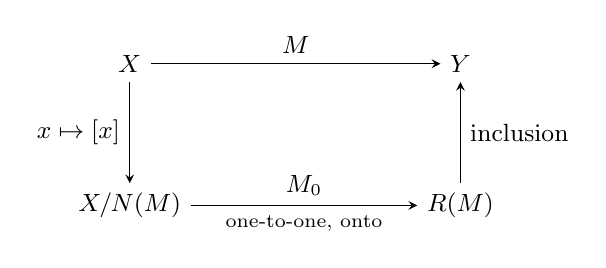
\begin{tikzpicture}[>=stealth, font=\small]
  \node (X) at (0,1.8) {$X$};
  \node (Y) at (4.2,1.8) {$Y$};
  \node (Q) at (0,0) {$X/N(M)$};
  \node (R) at (4.2,0) {$R(M)$};
  \draw[->] (X) -- node[above] {$M$} (Y);
  \draw[->] (X) -- node[left] {$x \mapsto [x]$} (Q);
  \draw[->] (Q) -- node[above] {$M_0$} node[below, font=\scriptsize] {one-to-one, onto} (R);
  \draw[->] (R) -- node[right] {inclusion} (Y);
\end{tikzpicture}
